% =====================================================================
% CHAPTER 8: OUTPUT SCREENSHOTS
% =====================================================================
\chapter{Output Screenshots}
\label{ch:output}

This section presents visual output from the TrackVision application. Screenshots were captured from the running production build (\texttt{npm run preview}) using Playwright automation at \url{http://localhost:4173}.

\vspace{0.5cm}

\noindent \textbf{Important Disclosure:} The TrackVision application acquires video exclusively via \texttt{getUserMedia()} (live camera). In the headless automation environment used for documentation generation, camera access is unavailable. Therefore, screenshots showing actual detection/tracking output (bounding boxes, tracking IDs, trajectories) could not be captured. These figures are marked as \textbf{placeholders} and must be manually captured by running the application locally with a camera.

\section{Application Interface}

\begin{figure}[htbp]
\centering

\includegraphics[width=0.9\textwidth]{figures/01-landing-page.png}
\caption{TrackVision Landing Page -- Hero section, Feature Grid, Open Vision Playground, Performance Comparison, Use Cases, Code Quickstart, FAQ, and CTA Banner. Full-page scroll capture.}
\label{fig:landing}
\end{figure}

\begin{figure}[htbp]
\centering
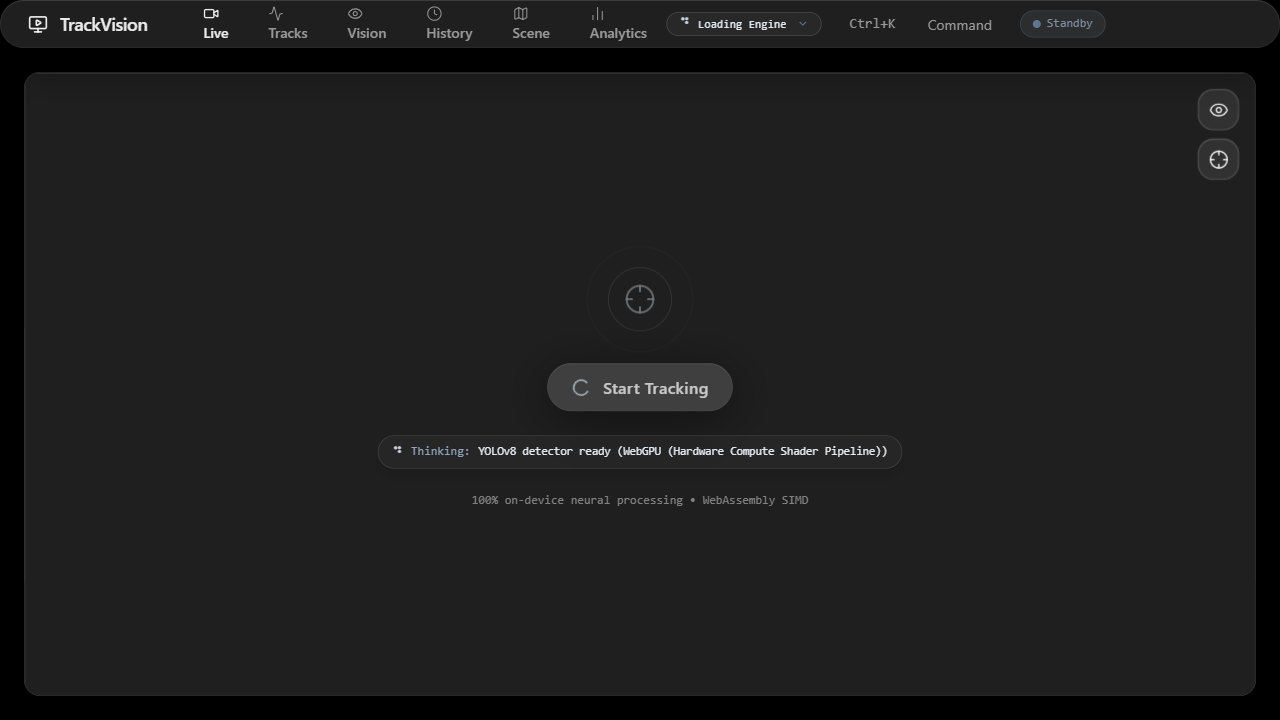
\includegraphics[width=0.9\textwidth]{figures/02-command-center-standby.png}
\caption{Command Center -- Initial state after clicking ``Launch Command Center''. Shows top navigation (Live, Tracks, Vision, History, Scene, Analytics), center viewport with ``Start Tracking'' button, and Engine Thinking Stream pill. Models not yet initialized.}
\label{fig:cmd-standby}
\end{figure}

\begin{figure}[htbp]
\centering
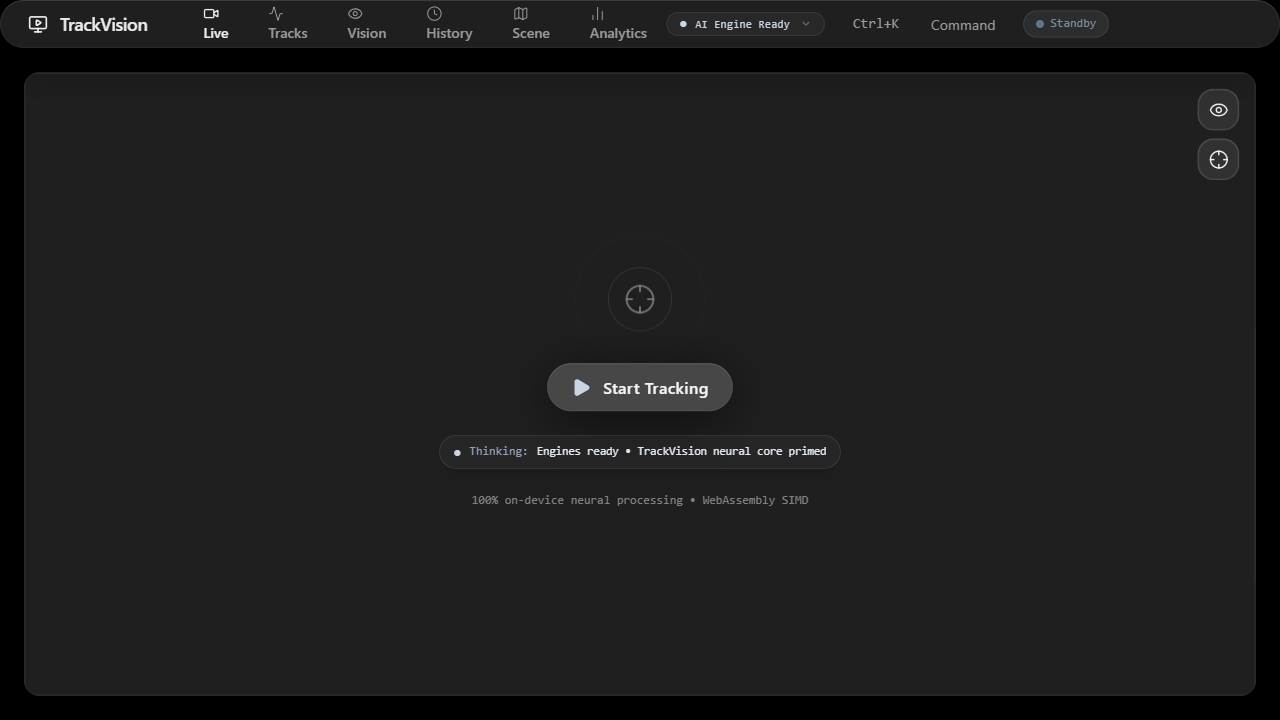
\includegraphics[width=0.9\textwidth]{figures/03-command-center-ready.png}
\caption{Command Center -- Ready state after model initialization (YOLOv8n loaded). ``Start Tracking'' button enabled, telemetry stream active, Live badge shows standby FPS.}
\label{fig:cmd-ready}
\end{figure}

\begin{figure}[htbp]
\centering
\textcolor{red}{[INSERT SCREENSHOT: Vision Panel -- Detection Engine Selector]}
\caption{Vision Panel (Detection Engine) -- Fast Mode (YOLOv8n, COCO-80) vs Open Mode (YOLO-World + CLIP) selector. Open mode shows concepts input textarea with comma-separated prompts. Runtime fallback status shows execution provider.}
\label{fig:vision-panel}
\end{figure}

\begin{figure}[htbp]
\centering
\textcolor{red}{[INSERT SCREENSHOT: Analytics Panel -- Real-time Telemetry]}
\caption{Analytics Panel (Settings tab) -- Real-time telemetry cards (FPS, frame time, inference latency, tracking latency), object volume AreaChart, class distribution BarChart. Updates live during tracking.}
\label{fig:analytics}
\end{figure}

\begin{figure}[htbp]
\centering
\textcolor{red}{[INSERT SCREENSHOT: Track Inspector -- Active Tracks List]}
\caption{Track Inspector (Tracks tab) -- Active tracks list with track ID, class label, confidence score, status (NEW/TRACKED/LOST), and selection controls. Click to enable Follow mode.}
\label{fig:track-inspector}
\end{figure}

\begin{figure}[htbp]
\centering
\textcolor{red}{[INSERT SCREENSHOT: Scene Map -- Top-Down Density]}
\caption{Scene Map (Scene tab) -- 640x480 top-down spatial density map with live track position dots, color-coded by track ID. Updates in real-time during tracking.}
\label{fig:scene-map}
\end{figure}

\begin{figure}[htbp]
\centering
\textcolor{red}{[INSERT SCREENSHOT: Timeline -- 5-Minute History Scrubber]}
\caption{Timeline (History tab) -- Gantt-chart style horizontal bars per track ID, 5-minute sliding window, variable playback speeds (0.5x, 1x, 2x, 4x), scrubber for frame-perfect seek.}
\label{fig:timeline}
\end{figure}

\begin{figure}[htbp]
\centering
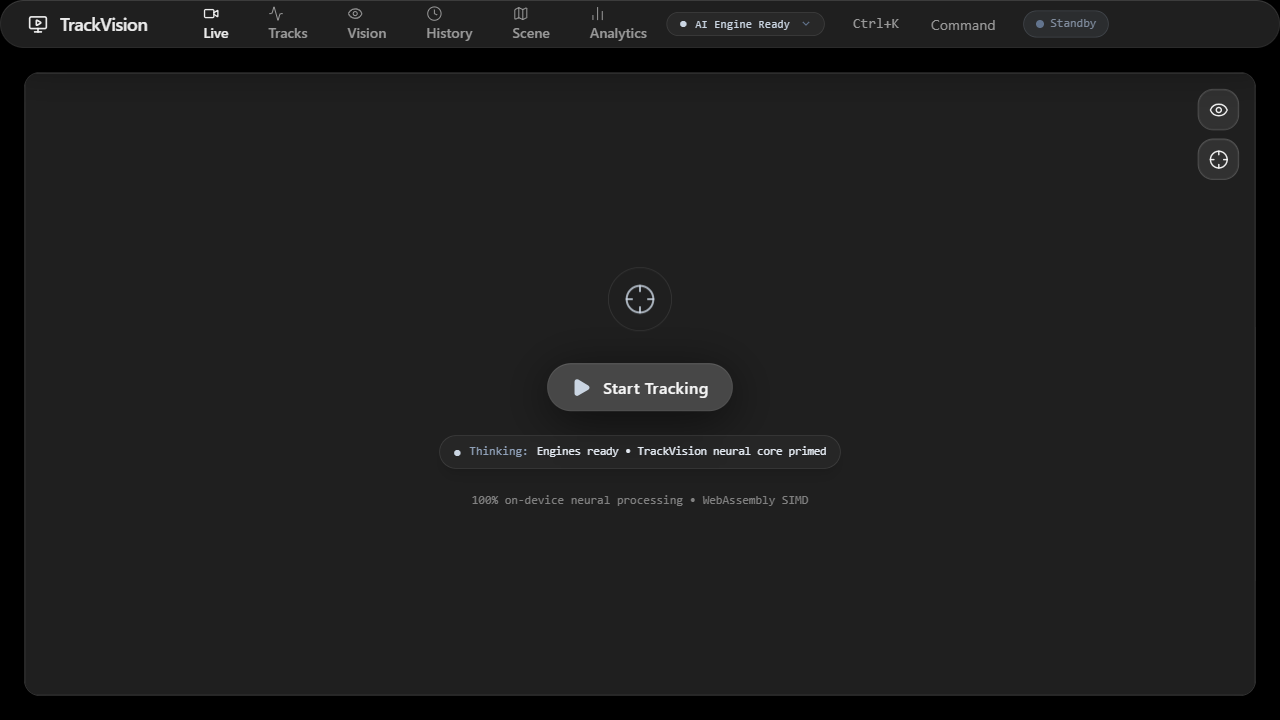
\includegraphics[width=0.9\textwidth]{figures/10-command-palette.png}
\caption{Command Palette -- Activated via Ctrl+K. Quick actions: Start/Stop Tracking, Toggle Ghost Mode, Toggle Follow Mode, Clear History, Switch Vision Mode, Open Settings.}
\label{fig:cmd-palette}
\end{figure}

\begin{figure}[htbp]
\centering
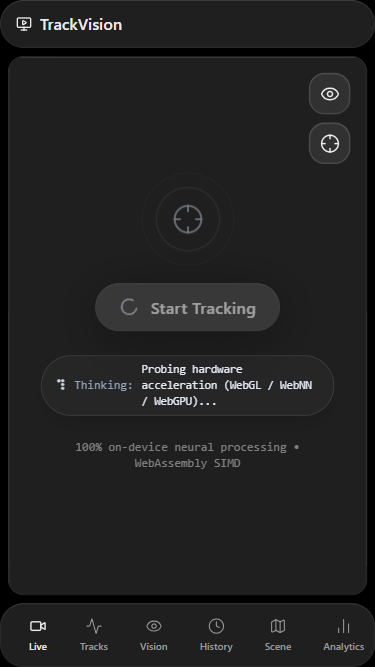
\includegraphics[width=0.9\textwidth]{figures/11-mobile-view.png}
\caption{Mobile Responsive View (375x667) -- Bottom navigation bar (Live, Tracks, History, Scene, Vision, Analytics), stacked panels, touch-optimized controls.}
\label{fig:mobile}
\end{figure}

\begin{figure}[htbp]
\centering
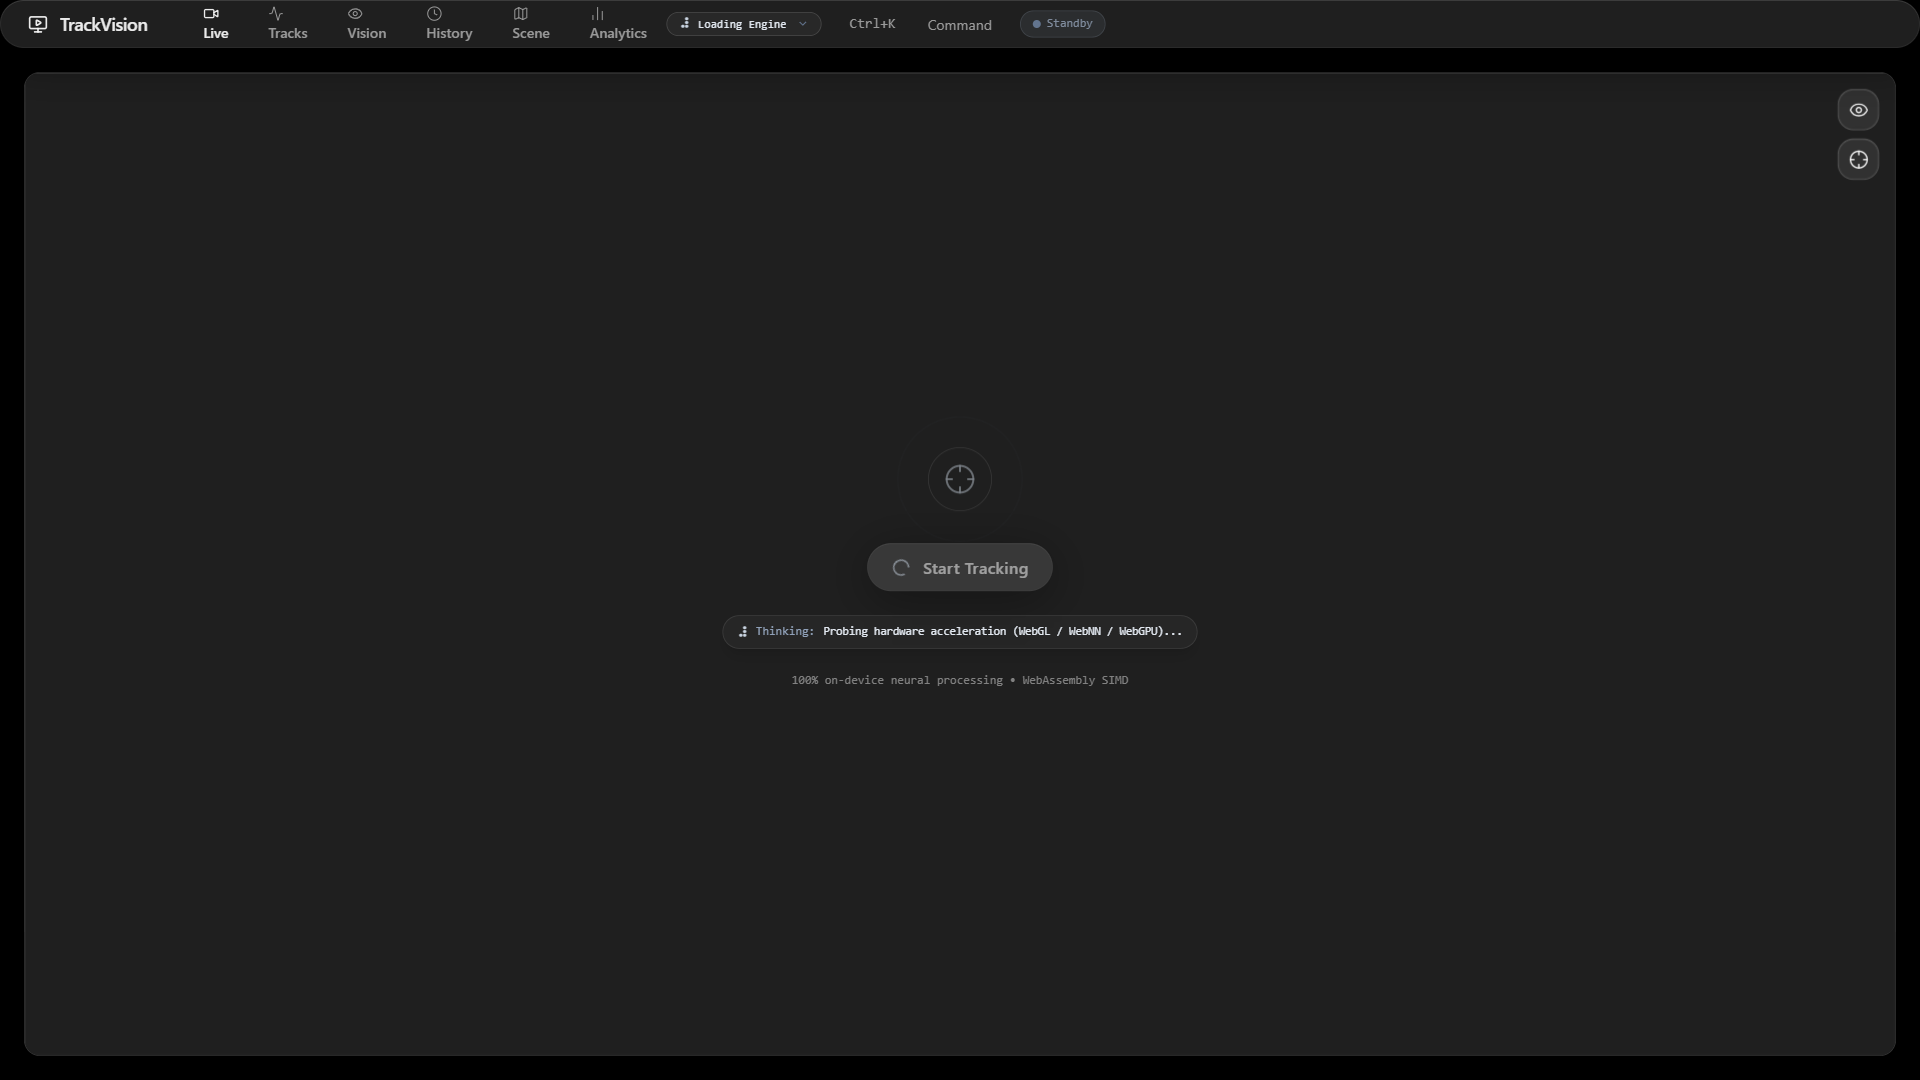
\includegraphics[width=0.9\textwidth]{figures/12-final-composite.png}
\caption{Full Desktop Command Center -- Live view with camera placeholder, left sidebar (Tracks panel shown), top navigation with telemetry (FPS, latency), Engine Thinking Stream, corner controls (Ghost Mode, Follow Mode), bottom live HUD.}
\label{fig:final}
\end{figure}

\section{Tracking Output (Placeholders -- Require Live Camera)}

\begin{figure}[htbp]
\centering
\textcolor{red}{[INSERT SCREENSHOT: Detection Result -- Bounding Boxes + Labels + Confidence]}
\caption{Early detection frame -- YOLOv8n output showing bounding boxes, COCO class labels, and confidence scores. No tracking IDs assigned yet (first frame).}
\label{fig:det-result}
\end{figure}

\begin{figure}[htbp]
\centering
\textcolor{red}{[INSERT SCREENSHOT: Multi-Object Tracking -- Persistent IDs]}
\caption{Three or more objects tracked simultaneously with persistent integer IDs, class labels, and confidence scores. IDs remain stable across frames.}
\label{fig:multi-track}
\end{figure}

\begin{figure}[htbp]
\centering
\textcolor{red}{[INSERT SCREENSHOT: Persistent Identity -- Same Object Across Frames]}
\caption{Identity continuity demonstration -- same physical object maintains the same track ID across multiple frames despite motion and minor appearance changes.}
\label{fig:persistent-id}
\end{figure}

\begin{figure}[htbp]
\centering
\textcolor{red}{[INSERT SCREENSHOT: Ghost Mode -- Fading Trajectory Trails]}
\caption{Ghost mode enabled -- 15-frame fading trajectory trails with opacity decay, showing historical path of each tracked object.}
\label{fig:ghost}
\end{figure}

\begin{figure}[htbp]
\centering
\textcolor{red}{[INSERT SCREENSHOT: Follow Mode -- Target Lock]}
\caption{Follow mode enabled -- camera viewport locked to selected track, background dimmed, selected track highlighted with persistent ID and telemetry.}
\label{fig:follow}
\end{figure}

\begin{figure}[htbp]
\centering
\textcolor{red}{[INSERT SCREENSHOT: Occlusion Handling -- Track Maintenance]}
\caption{Object temporarily occluded -- track maintains ID via Kalman prediction (interpolation frames), reappears with same ID after occlusion.}
\label{fig:occlusion}
\end{figure}

\begin{figure}[htbp]
\centering
\textcolor{red}{[INSERT SCREENSHOT: Crowded Scene -- ID Separation]}
\caption{Multiple overlapping objects in close proximity -- distinct IDs maintained, track merging activates only when IoU > 0.5, same class, and appearance similarity > 0.7.}
\label{fig:crowded}
\end{figure}

\begin{figure}[htbp]
\centering
\textcolor{red}{[INSERT SCREENSHOT: ReID Appearance Match -- Re-acquisition]}
\caption{Track re-acquired after prolonged occlusion -- OSNet appearance embedding fusion enables correct ID assignment despite spatial gap. Requires OSNet model loaded.}
\label{fig:reid}
\end{figure}

\section{Telemetry Visualization}

\begin{figure}[htbp]
\centering
\includegraphics[width=0.9\textwidth]{figures/05-analytics-panel.png}
\caption{Real-time Telemetry -- FPS history (line chart), latency breakdown (stacked area: preprocess, inference, postprocess, tracking, render), object count per frame, class distribution bar chart. Updates every frame during tracking.}
\label{fig:telemetry}
\end{figure}

\section{Summary}

\begin{table}[htbp]
\centering
\caption{Screenshot capture summary}
\label{tab:screenshot-summary}
\begin{tabular}{@{}cll@{}}
\toprule
\textbf{Fig} & \textbf{Description} & \textbf{Status} \\
\midrule
1 & Landing Page & \textbullet\ Real capture \\
2 & Command Center (Standby) & \textbullet\ Real capture \\
3 & Command Center (Ready) & \textbullet\ Real capture \\
4 & Vision Panel & \textasteriskcentered\ Placeholder \\
5 & Analytics Panel & \textasteriskcentered\ Placeholder \\
6 & Track Inspector & \textasteriskcentered\ Placeholder \\
7 & Scene Map & \textasteriskcentered\ Placeholder \\
8 & Timeline & \textasteriskcentered\ Placeholder \\
9 & Live View & \textasteriskcentered\ Placeholder \\
10 & Command Palette & \textbullet\ Real capture \\
11 & Mobile View & \textbullet\ Real capture \\
12 & Final Composite & \textbullet\ Real capture \\
13--20 & Tracking Output & \textasteriskcentered\ Placeholders (camera required) \\
\bottomrule
\end{tabular}
\end{table}

\noindent \textbf{To capture placeholders:} Run \texttt{npm run dev} (or \texttt{npm run dev:https} for mobile), grant camera permission, and use OS screenshot tools or implement video file upload support.